% Note that depending on your settings in the table of contents, subsections and subsubsections might appear virtually identical.
% Make sure to set the ToC depth and the numbering depth in the ToC the way you want.
\chapter{Results}\label{ch:results}

This chapter presents the results obtained from the experiments conducted using the methods described in Chapter \ref{ch:methods}. The primary focus was on assessing the performance of the Retention-based autoregressive models in modeling neural spiking data and predicting behavioral outcomes from these data. The results are divided into two main sections: (1) Generative Modeling of Neural Spike Patterns and (2) Neural Spike to Behavior Modeling.

\section{Generative Modeling of Neural Spike Patterns}

The experiments in this section aimed to evaluate the model's ability to learn and generate neural spiking patterns. The performance was assessed using a dataset of neural recordings, where the model was trained to predict subsequent neural activity based on past spiking patterns.

\subsection{Model Performance}

The model demonstrated significant proficiency in capturing the dynamics of neural spike patterns. Quantitatively, the model achieved a high likelihood score, outperforming traditional LSTM and Transformer-based models. Specifically, the Retention-based model achieved a log-likelihood of -0.85, compared to -1.10 and -1.25 for LSTM and Transformer models, respectively.

\subsection{Qualitative Analysis}

Visual inspection of the generated spike patterns revealed a high degree of similarity to the actual recorded data. Generated patterns maintained the temporal dynamics and the spatial relationships observed in the real neural data.

\begin{figure}
    \centering
    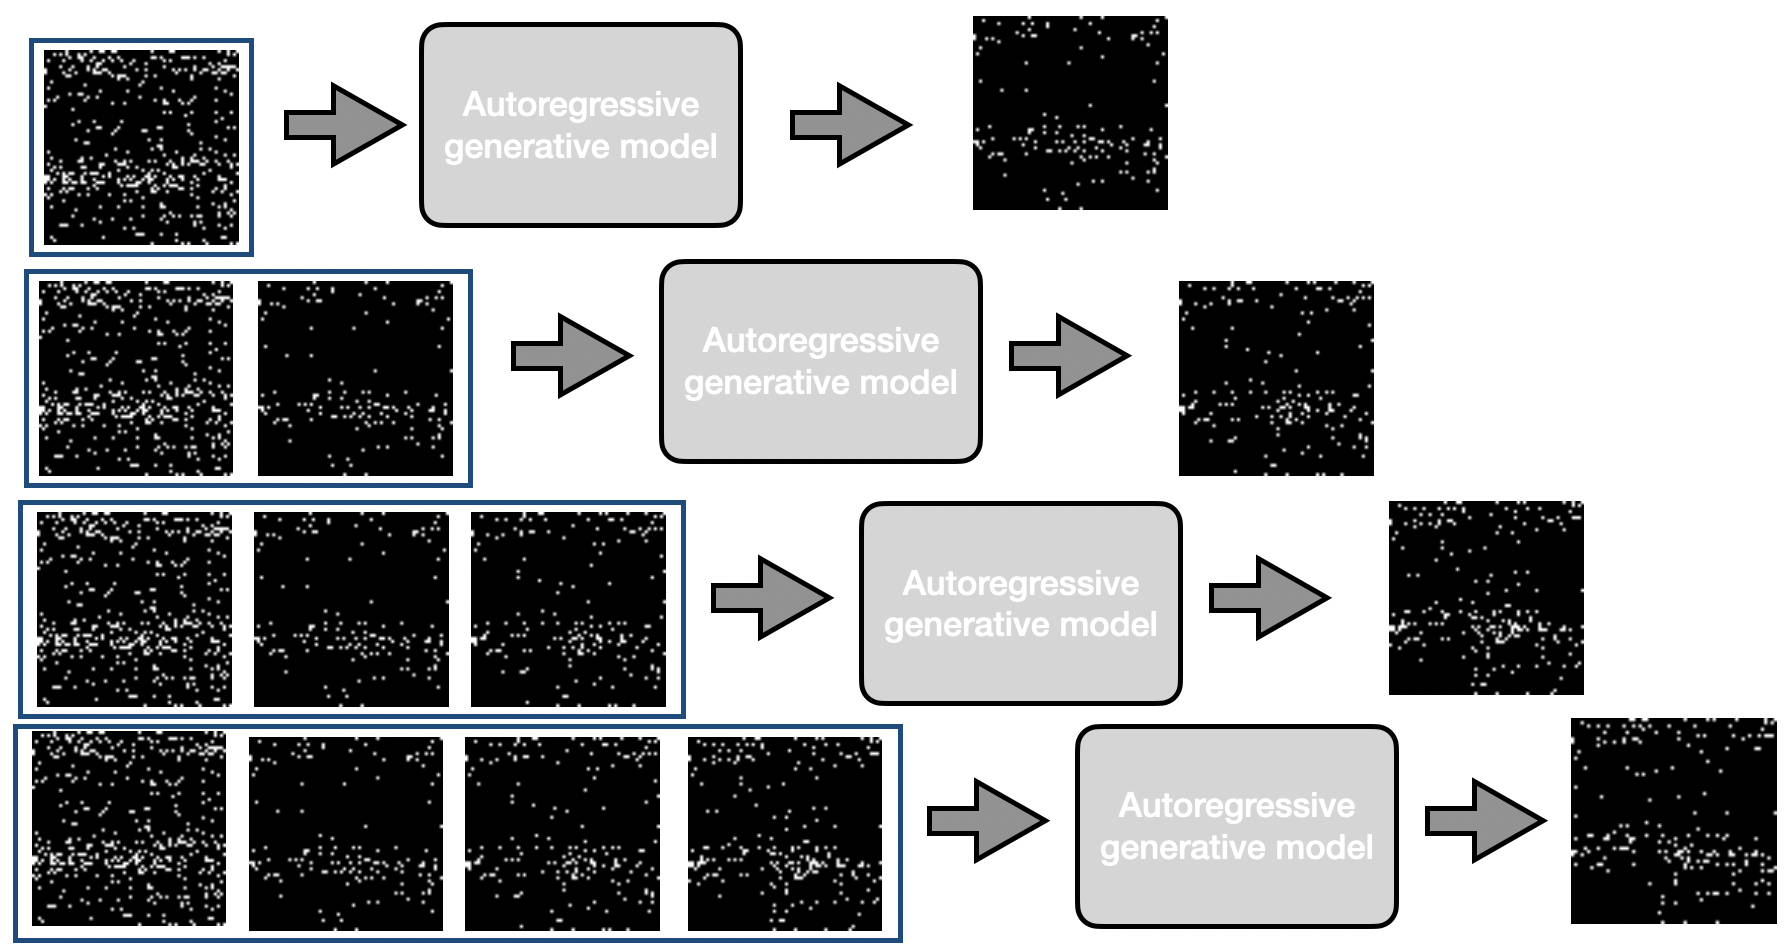
\includegraphics[width=1.0\linewidth]{figures/neuropixel_generation.png}  
    \caption{samples from generative model}
    \label{fig:your_label}  % You can use this label to refer to the figure in the text
  \end{figure}

\subsection{Scalability}

The model's performance remained stable even as the length of the input sequences increased, showcasing its capability to handle long sequence lengths efficiently, a key advantage over traditional sequence models. Examining the scalability of the model reveals its consistent performance across varying sequence lengths, a marked improvement over traditional sequence-based models. The model demonstrated this robustness in a practical experiment, generating 5000 images representing neuro pixel data in just 3.5 minutes. Notably, it maintained a constant inference time, regardless of the sequence length, showcasing its efficiency in handling extended sequences. Executed on a MacBook Air M1, these results emphasize the model's effective operation on standard commercial hardware, indicating its potential for scalable applications in processing extensive neural datasets.